\documentclass{article}

\usepackage{graphicx}
\usepackage[dvipsnames]{xcolor}
\graphicspath{ {.} }
\usepackage{siunitx}
\sisetup{load-configurations = abbreviations}
\usepackage{mathtools}
\usepackage{amsfonts}

\DeclarePairedDelimiter\ceil{\lceil}{\rceil}
\DeclarePairedDelimiter\floor{\lfloor}{\rfloor}
%\left( \right)
%\left\{ \right\}

\begin{document}
\section{Pôles et zéros}
\begin{enumerate}
\item
$$
x[n]=\left( \frac{1}{2} \right)^n \epsilon[n] + \left( \frac{1}{3} \right)^n \epsilon[n]
$$
Apply the Z-transform to both sides, using the property of linearity, and the z-transform table we obtain the following:

\begin{align}
  X(z) &= z\left\{ \left(\frac{1}{2}\right)^n \epsilon[n] \right\} + z\left\{ \left(\frac{1}{2}\right)^n \epsilon[n] \right\}  \nonumber\\
          &= \frac{1}{1-\left(\frac{1}{2}\right)z^{-1}} + \frac{1}{1-\left(\frac{1}{3}\right)z^{-1}} \nonumber\\
          &= \frac{2 -\frac{5}{6}z^{-1}}{\left(1 -\left(\frac{1}{2}\right) z^{-1}\right) \left(1 -\left(\frac{1}{3}\right) z^{-1} \right)}
\end{align}

Therefore, $X(z)$ has poles at $z=\frac{1}{2}$ and $z=\frac{1}{3}$ and a zero at $z=\frac{5}{12}$ \\

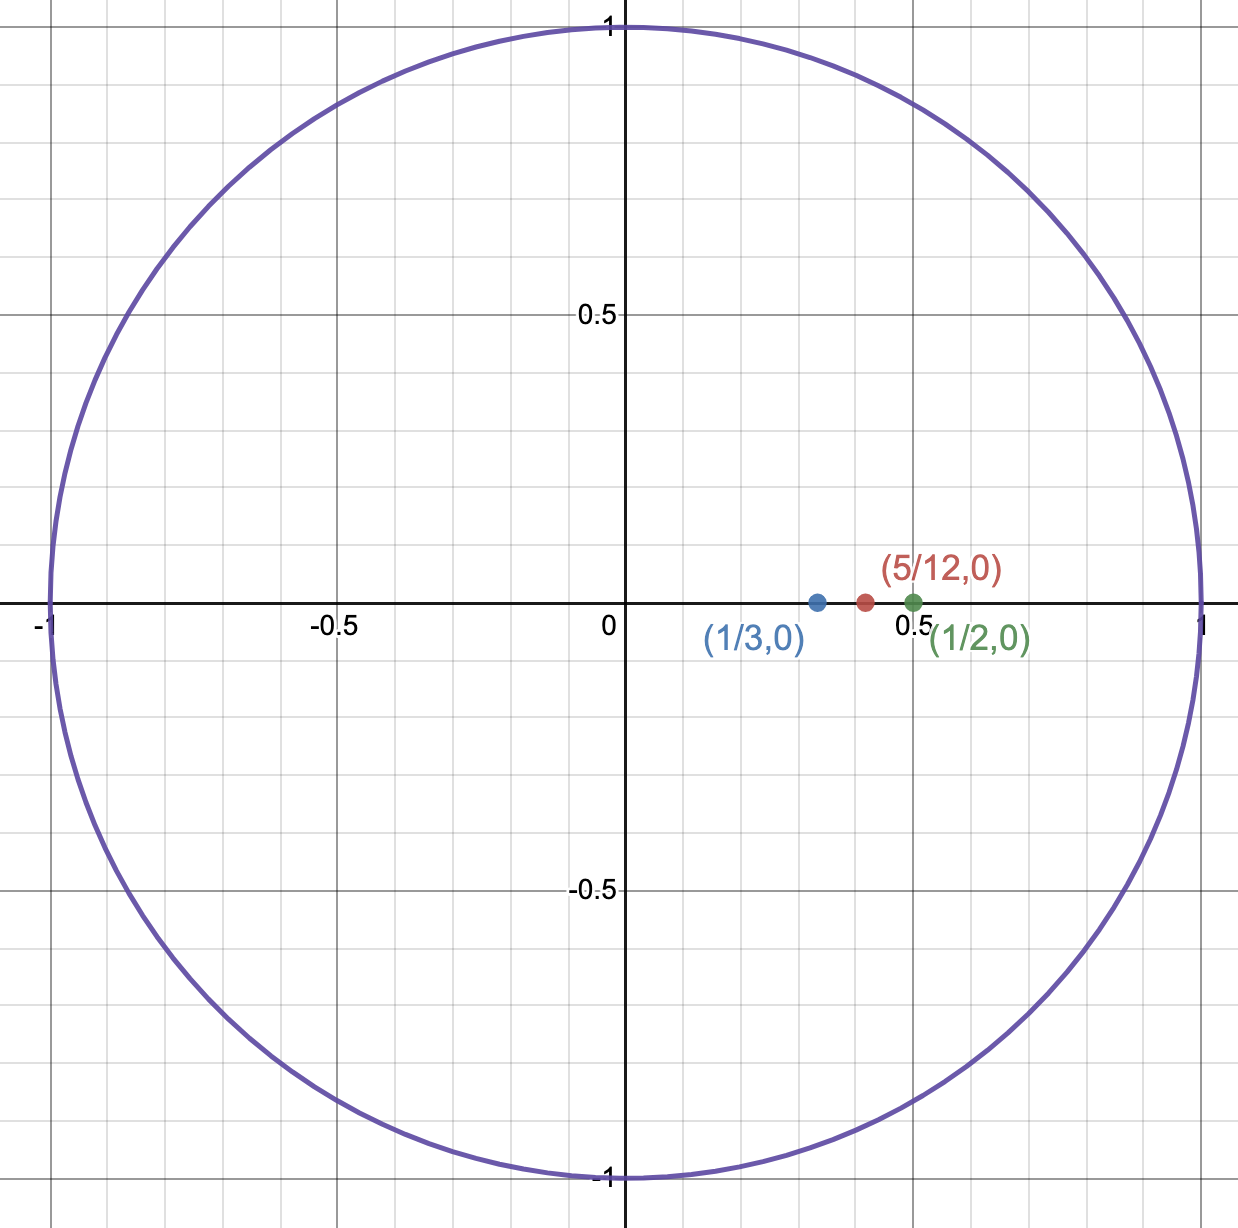
\includegraphics[width=170pt,height=170pt]{ee350_hw2_1_1} \\
The graph above represents the complex plane, with the y-axis as the imaginary axis, and the x-axis as the real axis

\item
\begin{enumerate}
\item
$$
x[n] =\left( \frac{1}{2}\right)^n\epsilon[n] - \left( \frac{1}{3}\right)^n\epsilon[-n-1]
$$
        Apply the z-transform to both sides, using the property of linearity of the z-transform (the final ROC of $X(z)$ will be the intersection of the ROCs of its constituent functions)
$$
   X(z) = z\left\{ \left(\frac{1}{2}\right)^n \epsilon[n] \right\} + z\left\{-\left(\frac{1}{3}\right)^n  \epsilon[-n-1] \right\}
$$

Using a z-transform table, we obtain the following expression

$$
X(z)= \frac{1}{1- \left( \frac{1}{2}\right) z^{-1}} + \frac{1}{1- \left( \frac{1}{3}\right) z^{-1}} = \frac{2 -\frac{5}{6}z^{-1}}{\left(1 -\left(\frac{1}{2}\right) z^{-1}\right) \left(1 -\left(\frac{1}{3}\right) z^{-1} \right)}
$$

The poles of found in 1.1 correspond to the ones found here. \\
However, the regions of convergence of the sub-functions $|z|> \frac{1}{2}$ and $|z| < \frac{1}{3}$ do not intersect, therefore, the region of convergence for $X(z)$ is $\emptyset$


\item
$$
x[n] =-\left( \frac{1}{2}\right)^n\epsilon[-n-1] - \left( \frac{1}{3}\right)^n\epsilon[-n-1]
$$
        Apply the z-transform to both sides, using the property of linearity of the z-transform (the final ROC of $X(z)$ will be the intersection of the ROCs of its constituent functions)
$$
   X(z) = z\left\{ -\left(\frac{1}{2}\right)^n \epsilon[-n-1] \right\} + z\left\{-\left(\frac{1}{3}\right)^n  \epsilon[-n-1] \right\}
$$

Using a z-transform table, we obtain the following expression

$$
X(z) = \frac{2 -\frac{5}{6}z^{-1}}{\left(1 -\left(\frac{1}{2}\right) z^{-1}\right) \left(1 -\left(\frac{1}{3}\right) z^{-1} \right)}
$$

The poles of found in 1.1 correspond to the ones found here. \\
The regions of convergence of the sub-functions $|z| < \frac{1}{2}$ and $|z| < \frac{1}{3}$ intersect, therefore, the region of convergence for $X(z)$ is $|z| < \frac{1}{3}$


\item

$$
x[n] =-\left( \frac{1}{2}\right)^n\epsilon[-n-1] + \left( \frac{1}{3}\right)^n\epsilon[n]
$$
        Apply the z-transform to both sides, using the property of linearity of the z-transform (the final ROC of $X(z)$ will be the intersection of the ROCs of its constituent functions)
$$
   X(z) = z\left\{ -\left(\frac{1}{2}\right)^n \epsilon[-n-1] \right\} + z\left\{ \left(\frac{1}{3}\right)^n  \epsilon[n] \right\}
$$

Using a z-transform table, we obtain the following expression

$$
X(z) = \frac{2 -\frac{5}{6}z^{-1}}{\left(1 -\left(\frac{1}{2}\right) z^{-1}\right) \left(1 -\left(\frac{1}{3}\right) z^{-1} \right)}
$$

The poles of found in 1.1 correspond to the ones found here. \\
The regions of convergence of the sub-functions $|z| < \frac{1}{2}$ and $|z| > \frac{1}{3}$ intersect, therefore, the region of convergence for $X(z)$ is $\frac{1}{3} < |z| < \frac{1}{2}$
\end{enumerate}
\end{enumerate}

\section{Transformée en $z$}
\begin{enumerate}
\item
$$
        x_1[n]= na^n\epsilon[n]
$$
        Let $y[n]= a^n\epsilon[n]$, from the z-transform table, we obtain $Y(z)= \frac{1}{1- az^{-1}}$\\
        We also have that the ROC of $Y(z)$ is $|z| > |a|$
        $$
        x_1[n]= ny[n]
        $$

        From the table of z-transforms we also have that given signal $x[n]$ with z-transform $X(z)$ and ROC $R$,\\
        the signal $nx[n]$ has z-transform $z\{nx[n]\}= -z\frac{dX(z)}{dz}$ and ROC $R$

        \begin{align}
         X_1(z) &= -z\frac{dY(z)}{z} \nonumber\\
                &= -z\frac{d}{dz}\left[ \frac{1}{1- az^{-1}}\right] \nonumber\\
                &= \frac{az}{(z-a)^2} \nonumber
        \end{align}

        The ROC of $x_1[n]= ny[n]$ is the same as the ROC of $Y(z)$, namely $|z| > |a|$

\item
$$
        x_2[n]= n^2a^n\epsilon[n]
$$
        From the problem 2.1, $x_1[n]= na^n\epsilon[n] \implies Y(z)= \frac{az}{(z-a)^2}$,
        and that the ROC of $X_1(z)$ is $|z| > |a|$

        $$
        x_2[n]= nx_1[n]
        $$

        From the table of z-transforms we also have that given signal $x[n]$ with z-transform $X(z)$ and ROC $R$,\\
        the signal $nx[n]$ has z-transform $z\{nx[n]\}= -z\frac{dX(z)}{dz}$ and ROC $R$

        \begin{align}
         X_2(z) &= -z\frac{dX_1(z)}{z} \nonumber\\
                &= -z\frac{d}{dz}\left[ \frac{az}{(z-a)^2}\right] \nonumber\\
                &= \frac{az(z +a)}{(z -a)^3} \nonumber
        \end{align}

        The ROC of $x_2[n]= nx_1[n]$ is the same as the ROC of $X_1(z)$, namely $|z| > |a|$
\item
    $$
        x_3[n]= a^n\cos(\omega_0n)\epsilon[n]
    $$
    Using the table of z-transforms we obtain the following:
    \begin{align}
        X_3(z) &= \sum_{k=-\infty}^{\infty} a^k\cos(\omega_0k)\epsilon[k]z^{-k} \nonumber \\
               &= \sum_{k=0}^{\infty} a^k\cos(\omega_0k)z^{-k} \nonumber \\
               &= \frac{1}{2} \sum_{k=0}^{\infty} \left( a^k\left( e^{j\omega_0k} +e^{-j\omega_0k} \right) \right)z^{-k} \nonumber \\
               &= \frac{1}{2}\sum_{k=0}^{\infty} a^ke^{j\omega_0k}z^{-k} + \frac{1}{2}\sum_{k=0}^{\infty} a^ke^{-j\omega_0k}z^{-k} \nonumber \\
               &= \frac{1}{2}\left( \frac{1}{1-ae^{j\omega_0}z^{-1}} + \frac{1}{1-ae^{-j\omega_0}z^{-1}} \right)= ... \nonumber \\
               &= \frac{1-[a\cos\omega_0]z^{-1}}{1-[2a\cos\omega_0]z^{-1}+a^2z^{-2}} \nonumber
    \end{align}

        The ROC of $X_3(z)$ is $|z| > a$
\end{enumerate}

\section{Transformée inverses}
\begin{enumerate}
\item
    $$
        X(z)= \frac{4z^{-1} + 1}{z^{-2} -3z^{-1} -10}
    $$
    By partial fraction decomposition, we obtain the following
    $$
        X(z)= \frac{4z^{-1} + 1}{(z^{-1}-5)(z^{-1}+2)}= \frac{3}{(z^{-1} - 5)} + \frac{1}{(z^{-1} + 2)} = X_1(z) + X_2(z)
    $$
         Where by the principle of linearity, the ROC of $X(z)$ will be the intersection of the ROCs of $X_1(z)$ and $X_2(z)$.\\

         Assuming that the system is causal, we obtain the following from examining the z-transform table

$$
    X_1(z) = \frac{3}{(z^{-1} - 5)} = \frac{-\frac{3}{5}}{1-\frac{z^{-1}}{5}} \implies  x_1[n]= -\frac{3}{5}\left( \frac{1}{5}\right)^n\epsilon[n]
$$
$$
    X_2(z) = \frac{1}{(z^{-1} + 2)} = \frac{\frac{1}{2}}{1 +\frac{z^{-1}}{2}} \implies x_2[n]=\frac{1}{2}\left( -\frac{1}{2}\right)^n\epsilon[n]
$$

$$
X(z) = X_1(z) + X_2(z) \implies x[n]= x_1[n] + x_2[n] = -\frac{3}{5}\left( \frac{1}{5}\right)^n\epsilon[n] + \frac{1}{2}\left( -\frac{1}{2}\right)^n\epsilon[n]
$$

        $X_1(z)$ has an ROC of $|z| > \frac{1}{5}$ and $X_2(z)$ has an ROC of $|z| > \frac{1}{2} $, therefore, $X(z)$ will have an ROC of $|z| > \frac{1}{2}$

\item
    \begin{align}
        X(z) &= cos(z^{-1}) \nonumber\\
             &= \frac{1}{2}\left( e^{jz^{-1}} + e^{-jz^{-1}}\right)
    \end{align}
    Substituing in the taylor series expansion of $e^x$ into the expression above we obtain the following:
    \begin{align}
        X(z) &= \frac{1}{2}\left( \sum_{k=0}^{\infty} \frac{(jz^{-1})^k}{k!}+ \sum_{k=0}^{\infty} \frac{(-jz^{-1})^k}{k!} \right)
             &= \sum_{k=0}^{\infty} \left( \frac{(1+(-1)^k)j^k}{2k!} \right)z^{-k}
    \end{align}

        From the definition of the z-transform: $X(z)= \sum_{k=-\infty}^{\infty} x(k)z^{-k}$ we obtain the following discrete-time function (where $\epsilon[n]$ is the unit-step function)

    \begin{align}
        x[n] &= \left( \frac{(1 +(-1)^k)j^k}{2k!}\right)\epsilon[n]
    \end{align}
\end{enumerate}

\section{La Fonction de Transfert}
\begin{enumerate}
\item
    \begin{align}
        y[n] &= x[n] -\frac{1}{2}x[n-1] + y[n-1] -\frac{1}{3}y[n-2] \nonumber\\
        Y(z) &= X(z) -\frac{1}{2}z^{-1}X(z) +z^{-1}Y(z) -\frac{1}{3}z^{-2}Y(z) \nonumber\\
        H(z) &= \frac{Y(z)}{X(z)}= \frac{1 -\frac{1}{2}z^{-1}}{1 -z^{-1} +\frac{1}{3}z^{-2}} \nonumber
    \end{align}

        Observing the z-transform table,
        $$
        z\left\{\left( r^n\cos\omega_0n\right)\epsilon[n]\right\} = \frac{1 -[r\cos\omega_0]z^{-1}}{1 -[2r\cos\omega_0]z^{-1} +r^2z^{-2}}
        $$

        Therefore, taking $r\cos\omega_0=\frac{1}{2} \implies r=\frac{\sqrt{3}}{3}$ and $\omega_0=\frac{\pi}{6}$, we also have that the ROC of $H(z)$ is $|z|> \frac{\sqrt{3}}{3}$\\

        Taking the inverse z-transform of $H(z)$ to determine the impulse response\\

    $$
    h[n]= \left(\frac{\sqrt{3}}{3}\right)^n\cos\left(\frac{\pi}{6}n\right)\epsilon[n]
    $$

\item
    $$
    y[n]= h[n] * \epsilon[n]
    $$

        Observing the table of z-transforms,
\begin{align}
    z\left\{x[n]\right\} &= X(z) \nonumber\\
    z\left\{\sum_{k=-\infty}^{n} x[k]\right\} &= \frac{1}{1-z^{-1}}X(z) \nonumber
\end{align}

        Using this property of the z-transform, and the property of the z-transform of a convolution

\begin{align}
 Y(z) &= H(z)\left(\frac{1}{1-z^{-1}}\right) \nonumber\\
    y[n] &= \sum_{k=-\infty}^{n} h[k] \nonumber\\
         &= \sum_{k=-\infty}^{n} \left(\frac{\sqrt{3}}{3}\right)^k \cos\left(\frac{\pi}{6}k\right)\epsilon[k] \nonumber
\end{align}

        The ROC of $y[n]$ in this case is at least $|z| > 1$

\item
    The system's output from an input of a step function $\epsilon[n]$ is the accumulation of the impulse response. Therefore for LTI systems, an input of $\delta[n]$ will yield the impulse response as an output, and an input of the step function $\epsilon[n]$ will yield the accumulation of said impulse response as an output.
\end{enumerate}

\end{document}
